
\chapter{Electroencephalography}
\section{Electricity in the brain}
As all known living organisms are composed of cells, so are humans and the human brain. The brain consists of nerve cells, or neurons, and non-neural cells, called glial cells. There are approximately 86 billion neurons in the human brain and roughly as much non-neural cells \cite{neuroncount}. A typical neuron has a cell body, multiple nerve endings, or dendrites, and one nerve fibre, or axon. Both, dendrites and axons can branch multiple times, but axons can be much longer than dendrites. 

There are connections between neurons, through which neurons can interact with each other by sending electro-chemical signals. These connections are not static and can change over time. Functionally related neurons are connected to each other and form neural pathways \cite{neuralpathway}. The general rule is that neuron sends signals through axon and receives signals through dendrites. The connection between an axon and a dendrite is called a synapse. 

\begin{figure}[h]
\centering
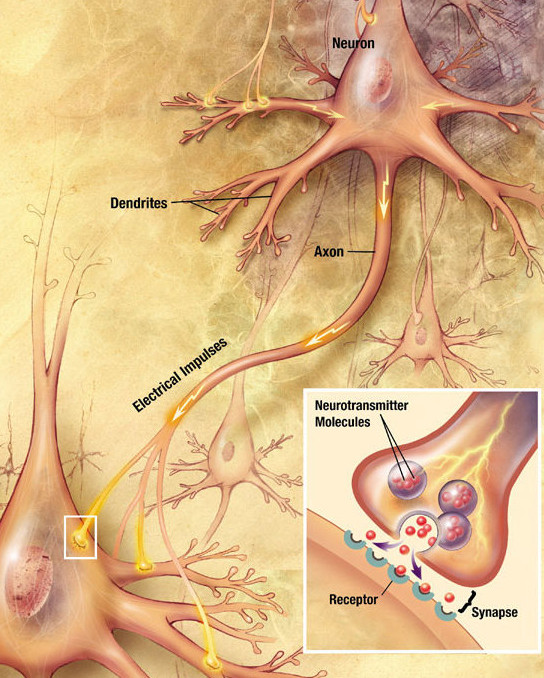
\includegraphics[width=0.5\textwidth]{synapse.jpg}
\caption{synapse caption\cite[p.~17]{neuronpic}}
\label{synapse}
\end{figure}

To send signals, neuron must be able to maintain electrical potential, called membrane potential. Membrane potential is defined as the difference in electric potential between the interior and exterior of a cell. When neurons are not sending signals, they have slightly negative membrane potential which is called resting potential. Negative resting potential is achieved by having more positively charged ions inside the cell than around it. The positively charged ions are sodium and potassium cations.

The concentration of potassium ions is higher in the interior of the cell, while the concentration of sodium ions is higher in the exterior. To maintain negative resting potential, the sodium-potassium pump is used. This pump transports three sodium cations out of the cell for every two potassium cations pumped in. Sodium-potassium pump is a active transport mechanism, which means that it moves ions across the cell membrane against their concentration gradient.

By having stable resting potential, neuron is able to send signals by rapidly increasing and decreasing the membrane potential along an axon.
This event is called an action potential and it is generated by voltage-gated ion channels, which are passive transport mechanisms. 

These channels are similar to sodium-potassium pumps but differ in the direction of ion transportation. Former is a active transport mechanism, meaning it moves ions across the cell membrane against their concentration gradient, while latter is passive transport mechanism which moves ions down the concentration gradient.

Voltage-gated ion channels, as the name suggests, are activated by a certain threshold voltage. When the membrane potential is near resting potential the channels are shut. 

A typical neuron fires 5 - 50 times every second.
 
\section{Recording brain activity}
\section{Visual evoked potentials}
 